\documentclass[12pt, oneside, smallheadings]{scrbook}

\usepackage[a4paper, reset, left=35mm,right=15mm, lines=46]{geometry}
\usepackage[utf8]{inputenc} % Umlaute ermöglichen
\usepackage[T1]{fontenc}
\usepackage[ngerman]{babel} % deutsche Silbentrennung
\usepackage[numbers,square]{natbib}
\usepackage{graphicx} % Grafiken
\usepackage[printonlyused]{acronym}
\usepackage{listings, marvosym}
\usepackage{url}
\usepackage{tabularx}
\usepackage{longtable}
\usepackage{array}
\usepackage{booktabs} 
\usepackage{todonotes}
\usepackage{xcolor}
\usepackage{subfigure} 
\usepackage{rotating}
\usepackage{multirow}
\usepackage{enumitem}
%\usepackage{dirtree}
\usepackage{textcomp}
\usepackage[htt]{hyphenat}

\definecolor{lbcolor}{rgb}{0.95,0.95,0.95}

\usepackage{minted}

\newcolumntype{R}[1]{>{\raggedleft\arraybackslash}p{#1}}                                                                                                                                                              
\newcolumntype{L}[1]{>{\raggedright\arraybackslash}p{#1}}                    

\usepackage[hidelinks]{hyperref}

\usepackage{bookmark}

\graphicspath{{img/}}
\makeatletter
\def\maxwidth#1{\ifdim\Gin@nat@width>#1 #1\else\Gin@nat@width\fi}
\makeatother
 
%%% Textart
\RequirePackage{lmodern}
\fontfamily{ptm}

%%% Zeilenabstand
\RequirePackage{setspace}  
\onehalfspacing

%%% Kopfzeile / Fußzeile
\RequirePackage[automark]{scrpage2}
\pagestyle{scrheadings}
\renewcommand\chaptermark[1]{
    \markboth{Kapitel \thechapter: #1}{}
}
\renewcommand\sectionmark[1]{
    \markright{#1}
}
\clearscrheadfoot
\setheadsepline{0.4pt}
\ihead{\footnotesize\textnormal\leftmark}
\chead{}
\ohead{\footnotesize\textnormal\rightmark}

\ifoot{}
\cfoot[\pagemark]{\textnormal{\thepage}}
\ofoot{}
%%% Ende Kopfzeile / Fußzeile

%%% Referenzen
\RequirePackage{prettyref}
\RequirePackage{titleref}

% Kapitel
\newrefformat{chap}{siehe Kapitel \ref{#1}, Seite \pageref{#1}}
% Abschnitte
\newrefformat{sec}{siehe Abschnitt \ref{#1}, Seite \pageref{#1}}
% Abbildungen
\newrefformat{fig}{siehe Abbildung \ref{#1}}
% Tabellen
\newrefformat{tab}{siehe Tabelle \ref{#1}}
% Listings
\newrefformat{lst}{siehe Listing \ref{#1}}

\newcommand{\pref}[1]{\prettyref{#1}}
\newcommand{\siehe}[1]{\prettyref{#1}}
%%% Ende Referenzen

%%% Beeinflusst die Eintragungen im Inhaltsverzeichnis
%\AtBeginDocument{\addtocontents{toc}{\protect\thispagestyle{empty}}} 

%%% Glossar
\usepackage[acronym, toc, style=long, nonumberlist, nomain]{glossaries}
%Glossar-Übersetzungen:
\RequirePackage{glossaries-babel}
\newcommand{\abk}[1]{\gls{#1}}

%\newacronym[]{KEY}{SHORT}{LONG}
%A
\newacronym[]{aal}{AAL}{Amient Assisted Living}
%B
%C
%D
%E
%F
%G
%H
%I
%J
%K
%L
%N
\newacronym{nfc}{NFC}{Near Field Communication\glsadd{nfcg}}
%M
%O
%P
\newacronym{pir}{PIR}{Passive Infrared}
%Q
%R
\newacronym{rfid}{RFID}{Radio Frequency Identification}
%S
\newacronym{sdk}{SKD}{Software Development Kit}
%T
\newacronym{tts}{TTS}{Text-To-Speech}
%U
\newacronym{uv}{UV}{Ultraviolett}
\newacronym{ui}{UI}{User Interface}
%V
%W
\newacronym{whz}{WHZ}{Westsächsische Hochschule}
%X
%Y
%Z


%%%%%%%%%%%%%
%  GLOSSAR  %
%%%%%%%%%%%%%
\makeglossaries

%\newglossaryentry{...}
%{
%  name=SOAP,
%  description={...}
%}
%%% Ende Glossar

%%% Style Listings
\usepackage{chngcntr}% http://ctan.org/pkg/chngcntr
\counterwithin{listing}{chapter}

\begin{document}

%%% Einrücken bei neuen Absatz verhindern
%\setlength{\parindent}{0pt}

%%% Titelseite
\pdfbookmark[0]{Titelseite}{titlepage}
\begin{titlepage}
	\vspace*{5mm}
	\begin{center}
%		\includegraphics[scale=1]{images/z-wave-logo.png}\\
		\vspace*{3cm}
		\Large
		\textbf{Projekt im Master}\\
		\vspace*{3cm}
		\Huge
		\textbf{Projektdokumentation}\\
		\vspace*{3cm}
	
		\vfill
		\normalsize
		\newcolumntype{x}[1]{>{\raggedleft\arraybackslash\hspace{0pt}}p{#1}}
		\begin{tabular}{x{6cm}p{7.5cm}}
			\rule{0mm}{5ex}\textbf{Autoren:} & Patrick Hecker\newline Patrick.Hecker.1kg@fh-zwickau.de \\ 
			\rule{0mm}{5ex}					 & Simon Schwabe\newline Simon.Schwabe.1su@fh-zwickau.de \\ 
			\rule{0mm}{5ex}\textbf{Projektleiter:} & Prof. Dr Golubski \\ 
			\rule{0mm}{5ex}\textbf{Datum:} & \today \\ 
		\end{tabular} 
	\end{center}
\end{titlepage}


\setcounter{page}{1}
\setcounter{tocdepth}{1}
\pagenumbering{roman}

%%% Inhaltsverzeichnis
\clearpage
\pdfbookmark[0]{Inhaltsverzeichnis}{contents}
\tableofcontents
\thispagestyle{plain}

%%% Glossar (Abkürzungen)
\printglossary[type=\acronymtype, title=Akronymverzeichnis,toctitle=Akronymverzeichnis]
% \printglossary[title=Glossar,toctitle=Glossar]

%%% Tabellenverzeichnis
% \listoftables
% \addcontentsline{toc}{chapter}{Tabellenverzeichnis}

%%% Abbildungsverzeichnis
% \listoffigures
% \addcontentsline{toc}{chapter}{Abbildungsverzeichnis}

%%% Listingsverzeichnis
%\renewcommand\listoflistingscaption{Listingverzeichnis}
%\listoflistings
%\addcontentsline{toc}{chapter}{Listingverzeichnis}

%%% Inhalt
\clearpage
\pagenumbering{arabic}
\setcounter{page}{1}

\pagestyle{scrheadings}

\chapter{Einleitung} 
\begin{itemize}
	\item Zeitrahmen des Projekts
	\item Mitarbeiter, Verantwortlichkeiten
\end{itemize}

\chapter{Projektziel}
\begin{itemize}
	\item aktueller Stand (Ist-Analyse)
	\item Gegenstand, Motivation, Zielstellung des Projekts
\end{itemize}

\chapter{Vorgehensplan}
\begin{itemize}
	\item grober Vorgehensplan, um "`Big Picture"' nicht aus den Augen zu verlieren
	\item agiles Vorgehen

\end{itemize}

\chapter{Projektverlauf}
\begin{itemize}
	\item welche konkreten Aufgaben wurden wann bearbeitet
	\item Verweise auf Arbeitsergebnisse
\end{itemize}

\section{Sprint 1}
\begin{itemize}
	\item Zeitraum: 02.10.15 - 09.10.15
	\item Task \#3866: Einarbeitung
\end{itemize}
Am 02.10.15 fand das initiale Projektmeeting statt. In einem Vortrag für die Projektmitglieder wurde die Thematik Smart Home im Allgemeinen und Z-Wave als Kommunikationsprotokoll im Speziellen vorgestellt. Dadurch sollten Kenntnisse und Wissensstand der Teammitglieder auf ein einheitliches Niveau gehoben werden. Die verschiedenen Rollen der Mitglieder im Projekt wurden verteilt und ein organisatorischer Rahmen festgelegt.

Da es sich um ein Projekt mit erheblichem Forschungsanteil handelt, fiel die Entscheidung auf agiles Vorgehen und gegen eine starre Projektplanung im Voraus. Im Rahmen des Projekts wird mit Sensoren gearbeitet und zum Zeitpunkt der Initialisierung liegen noch wenige konkrete Erfahrungen im Umgang und zur Leistungsfähigkeit der Sensoren vor.

Ziel des Sprints ist eine selbstständige, vertiefende Einarbeitung in die Thematik. Dieses Wissen bildet die Diskussionsgrundlage für das weitere Vorgehen.

\section{Sprint 2}
\begin{itemize}
	\item Zeitraum: 09.10.15 - 16.10.15
	\item Task \#3883: Multi-Personen Szenarien erarbeiten
	\item Task \#3885: Szenarien erstellen \& diese mittels Z-Wave Komponenten realisieren
\end{itemize}

\section{Sprint 3}
\begin{itemize}
	\item Zeitraum: 16.10.15 - 23.10.15
	\item Task \#3933: Sensorauswahl für die favorisierten Szenarien
	\item Task \#3960: Modellierung der Szenarien
	\item Task \#3961: Szenarien nacharbeiten
\end{itemize}

\section{Sprint 4}
\begin{itemize}
	\item Zeitraum: 23.10.15 - 30.10.15
	\item Task \#3961: Szenarien nacharbeiten
	\item Task \#4007: Modelle nacharbeiten
	\item Task \#4010: Konzept für Module entwickeln
	\item Task \#4012: Feedbackmöglichkeiten erarbeiten
	\item Task \#4013: Versuchsaufbau konzipieren
\end{itemize}

Während des vierten Sprints wurden die ausgewählten Szenarien und daraus resultierenden Modelle nochmals überarbeitet und konkretisiert. 
%TODO auf Resultate verweisen
Die Erweiterung der bestehenden Serveranwendung ist durch Module möglich. Anhand der erarbeiteten Szenarien wurden zu entwickelnde Module konzipiert und die Wechselwirkung zwischen verschiedenen Modulen analysiert. Außerdem wurde ein "`Hello World"' Modul zur Verfügung gestellt, um einen Einblick in die Modulentwicklung zu gewähren.

\section{Sprint 5}
\begin{itemize}
	\item Zeitraum: 30.10.15 - 06.11.15
	\item Task \#4010: Konzept für Module entwickeln
	\item Task \#4012: Feedbackmöglichkeiten erarbeiten
	\item Task \#4013: Versuchsaufbau konzipieren
	\item Task \#4065: Einarbeitung "`Entwicklung von Z-Way Modulen"'
\end{itemize}
Ziel dieses Sprints war die Einarbeitung in die Modulentwicklung für den Z-Way-Server. Dazu wurden zwei HelloWorld-Module zur Verfügung gestellt. Ein minimales Beispiel verdeutlichte die grundlegende Entwicklung von Modulen ohne großen Funktionsumfang. Das zweite Modul bot einen erheblich erweiterten Funktionsumfang und bot somit tiefere Einblicke in die Entwicklung für den Z-Way-Server. Während eines Meetings der gesamten Projektgruppe wurde das minimale Beispiel Schritt für Schritt zu dem umfangreichen Modul ausgebaut um ein Gefühl für die Entwicklung zu vermitteln. Behandelte Themen waren unter anderem das Senden und Empfangen von Events über den Eventbus, die Konfiguration von Modulen mittels Alpaca.js und die Bereitstellung von Funktionen über die ZAutomation-API.

\section{Sprint 6}
\begin{itemize}
	\item Zeitraum: 06.10.15 - 13.11.15
	\item Task \#4012: Feedbackmöglichkeiten erarbeiten
	\item Task \#4013: Versuchsaufbau konzipieren
\end{itemize}

\chapter{Arbeitsergebnisse}
\begin{itemize}
	\item Ergebnisse, welche für den weiteren Verlauf relevant sind (z.B. zu realisierende Szenarien)
	\item weiterverfolgte Szenarien
\end{itemize}

\section{Szenarien}

\subsection{Effizienz und Komfort - Erkennung der Anzahl der Personen in einem Raum}
\subsubsection{Ablauf}
Person A geht zusammen mit Person B vom Flur in das Wohnzimmer, während Person C in die Küche geht.
Die Lichter werden im Flur deaktiviert, im Wohnzimmer und in der Küche aktiviert.
Person D betritt die Wohnung und wird von den Personen A und B in der Tür zum Wohnzimmer begrüßt. Zusammen gehen sie ins Wohnzimmer.
Dabei werden zunächst die Lichter im Flur erneut aktiviert und nach der Begrüßung wieder deaktiviert.
Nach einiger Zeit ruft Person D zum Essen und es verlassen Personen A, B und C das Wohnzimmer und gehen in die Küche.
Sobald die letzte Person das Wohnzimmer verlassen hat werden die Lichter im Wohnzimmer deaktiviert.

\subsubsection{Erforderliche Komponenten}
\begin{itemize}
	\item ZWay Steuereinheit
	\item 2 x Bewegungsmelder / Fibaro 6-in-1 Sensor pro Tür
	\item Modul zur Lichtersteuerung
\end{itemize}

\subsubsection{zur Diskussion}
Unbekannt ob Begrüßungssituation ausreichend abgegrenzt werden kann, ohne Fehler hervorzubringen.
Tür könnte zusätzlich mit Türsensor ausgestattet werden um ein Durchgehen zu bestätigen bzw. vorbeigehende Personen bei geschlossener Tür zu ignorieren.

\subsubsection{Modelle}
%TODO textuelle Beschreibung der Modelle
\begin{figure}[h!]
	\centering
	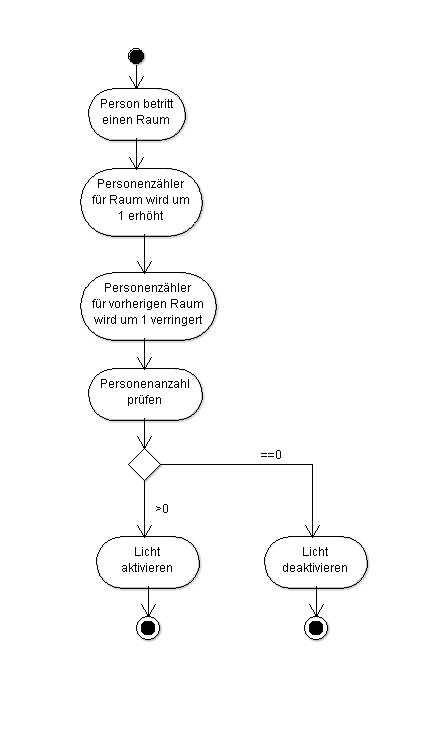
\includegraphics[scale=1]{img/Szenarien/Effizienz_Komfort_Erkennung_Anzahl_Personen.png}
	\caption{Erkennung Anzahl Personen}
	\label{fig:szenarienPersonenerkennung}
\end{figure}

\begin{figure}[h!]
	\centering
	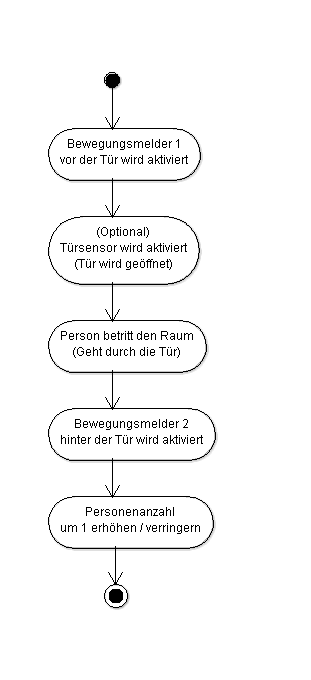
\includegraphics[width=0.9\textwidth]{img/Szenarien/Personenerkennung_an_Tuer.png}
	\caption{Personenerkennung an der Tür}
	\label{fig:szenarienPersonenerkennungTür}
\end{figure}


\subsection{Haus bei verschließen der Haus- Wohnungstür in "`Standby"' versetzen}
\subsubsection{Ablauf}
Um den Komfort in ihrem Smart Home zu steigern, möchte Anne möglichst wenig Aufwand zur Steuerung des Lichts betreiben. Dazu möchte sie bei Verlassen der Wohnung nicht alle angeschalteten Lampen manuell ausschalten und überprüfen, ob Gefahrenquellen vom Stromnetz getrennt sind.

Ein intelligentes, vernetztes Türschloss überträgt dazu beim Abschließen der Wohnung ein entsprechendes Signal an die zentrale Steuereinheit. Diese Steuereinheit interpretiert das Signal und schaltet alle Lampen aus. Außerdem werden vorher konfigurierte Steckdosen deaktiviert, um das Brandrisiko zu minimieren. Damit wird die Wohnung in einen "`Standby-Modus"' versetzt. Auch in diesem Fall möchte Anne nicht alle Geräte vom Stromnetz trennen, ihr Laptop soll weiterhin mit Strom versorgt und der Akku geladen werden.

Befindet sich Tom noch in der Wohnung, wenn sie abschließt, soll er nicht durch die Steuerung gestört werden. Das heißt in diesem Fall wird die automatische Abschaltung nicht durchgeführt. Dazu ist es notwendig, dass verschiedene Sensoren des Systems zuverlässig erkennen, ob Personen anwesend sind. Die automatische Steuerung wird erst aktiv, wenn der letzte Bewohner die Wohnung verlässt und abschließt.

\subsubsection{zur Diskussion}
\begin{itemize}
	\item welche Komponenten sind von Abschaltung betroffen (z.B. Lampen, Steckdosen von Wasserkocher, Kaffeemaschine, ...)
	\item welche Komponenten sind ausgeschlossen (z.B. Kühl- und Gefrierschränke, Waschmaschinen, ...)
\end{itemize}

\subsubsection{erforderliche Komponenten}
\begin{itemize}
	\item Steuereinheit
	\item vernetztes Türschloss
	\item Sensoren zu Personenerkennung: z.B. Bewegungsmelder, Infrarot, 
	\item schaltbare Steckdosen, evtl. mit Verbrauchserkennung
	\item schaltbare Lampen
\end{itemize}

\subsubsection{Modellierung aus Systemsicht}

\subsubsection{Modellierung aus Nutzersicht}



\chapter{Fazit}
% Ausblick, weiteres Vorgehen
\begin{itemize}
	\item Bewertung der Projektergebnisse
	\item Ausblick, Erweiterungsmöglichkeiten
\end{itemize}

\newpage

%\chapter{Einleitung}
%\label{chap:einleitung}
%Dieses Dokument soll eine Hilfestellung bei der Arbeit mit dem Funkprotokoll Z-Wave und dem Z-Way-Server sein. Zu Beginn (\prettyref{sec:z-wave}) wird ein kurzer Überblick über das Funkprotokoll Z-Wave gegeben. Für eine detailliertere technische Beschreibung des Standards sei auf das Z-Wave-Vademekum von Dr. Pätz verwiesen \cite[]{Pae14}.
%
%Etwas umfangreicher wird die Installation, Architektur und User Interface des Z-Way-Servers beschrieben. Der letzte Teil des Dokuments beschreibt die Nutzung der Z-Way-API und die Erweiterung der Serverfunktionalität durch die Entwicklung zusätzlicher Module.
%
%\begin{figure}[h!]
%	\centering
%	\includegraphics[width=0.9\textwidth]{images/what-is-zwave.jpg}
%	\caption{What is Z-Wave? \cite{WhatIsZWave}}
%	\label{fig:zway-ui}
%\end{figure}

%%% Quellenverzeichnis
%\renewcommand{\bibname}{Quellenverzeichnis}
%\bibliography{literature/literature}{}
%\addcontentsline{toc}{chapter}{\bibname}
%\bibliographystyle{alphadin} %natdin

%%% Anhang
\appendix
\addtocontents{toc}{\protect\contentsline{chapter}{Anhang}{}{}}

\chapter{Protokolle der Meetings}
\label{[chap:protokolle]}

\section{1. Treffen (02.10.15)}
\begin{itemize}
	\item bisherige Steuerung/Kontrolle von Smart-Home Geräten im Haus durch simple Zeit-/Anwesenheitssteuerung
	\item Probleme und Vorgaben:
	\begin{itemize}
		\item Beeinflussung des Systems von einer zweiten Person zur gleichen Zeit
		\item momentan existieren nur eine Person Steuerungskonzepte
		\item erarbeiten von Konzepten für mehrere Personen
		\item Wechselwirkung in der Beeinflussung des Systems z.B.: äußere Person beeinflusst Dinge die anwesende Person/en beeinflussen
		\item Besprochene Beispiele Jalousie-Schaltung, Feuermelder
		\item (Feedback von Systemänderungen an die Anwesenden Person) Feedback an Auslöser des Ereignisses
		\item Feedback über eingebaute Geräte Licht/Audio Effekte eventuell
		\item Interaktion durch Signale und vorhandene Schalter etc.
		\item Generationenkonflikt daher nicht Telefon/Smartphone fest anbinden
		\item geringe Kosten Massenmarkt/Low-Budget Bereich
		\item ZUno Projekt
	\end{itemize}
	
	\item Kreativität gefragt
	\item Ziel: Idealfall Szenarien mit praktischer Demonstration, sodass präsentierbar
	\item Analyse des Systems
	\item Z-Wave.eu \textrightarrow Hohenstein
	\item Z-Wave.me \textrightarrow Schweiz, Deutschland, Russland
	\item ZWay \textrightarrow Softwarepaket/Server
	\item Hersteller übergreifende Kommunikation
	\item Simulation möglich
	\item mögliches Vorgehen: Recherche für Sensoren
	\item Android oder Webapp möglich (Teil von ZWay)
	\item Informationen durch die Foren
	\item Entwicklung zwei bis drei Szenarien das Mehr-Personen-Steuerung notwendig
	\item Vortrags-links werden bereitgestellt
	\item Organisatorisches
	\begin{itemize}
		\item Redmine Projekt
		\item Scrum
	\end{itemize}
\end{itemize}

\section{2. Treffen (09.10.15)}
\begin{itemize}
	\item Vortrag siehe Folien (Redmine)
	\begin{itemize}
		\item mehrere überlappende Netzwerke, wie ist das realisiert
		\item Gruppenarbeit Sensorrecherche bis nächste Woche
		\item Sensoren allgemein
		\item Aktivität anhand des Stromverbrauchs erkennen, Fensterkontakt
		\item weitere Technologien, die evtl. in Betracht gezogen werden können: Beacon, Z-Uno, RFID, NFC
		\item zusätzliche Informationsquellen einbinden, und so mehr über einen typischen Tagesablauf lernen, z.B. Terminkalender
		\item Vorstellung der Smart Home UI
		\item Frage ob Z-Uno gebraucht wird oder nicht
		\item was mit dessen Hilfe realisierbar ist
		\item Raspberry Pi bzw. Funkmodul (RaZberry besorgen)
		\item Z-Wave Programmierumgebung über Z-Wave oder JavaScript
	\end{itemize}
		
	\item Besprechung
	\begin{itemize}
		\item Sensorensuche
		\item Sensoren intelligent vernetzen
		\item Liste mit Sensoren (Z-Wave Europe)
		\item wie wird das mit einem Modell oder Raum
		\item wie können Erkenntnisse anschaulich vermittelt werden
		\item 2 Gruppen die jeweils 3 bis 5 Szenarien erarbeiten
		\item Gruppeneinteilung
	\end{itemize}
\end{itemize}
\section{3. Treffen (16.10.15)}

\begin{itemize}
	\item Vorstellung der in Gruppen erarbeiteten Szenarien
	\item Gruppe 1:
	\begin{itemize}
		\item Sicherheit im Heim durch Abschaltung von Gefahrenquellen (z.B. Haartrockner) bei Verlassen der Wohnung
		\item Gefahrenquellen (z.B. Ofen) deaktivieren, wenn keine Erwachsenen anwesend sind
	\end{itemize}
	\item Gruppe 2:
	\begin{itemize}
		\item Personenzähler je Raum anlegen, entsprechend der Personenanzahl unterschiedliche Aktionen ausführen
		\item Personenerkennung an der Tür durch außen und innen angebrachten Bewegungsmelder, evaluieren, wie zuverlässig diese Sensoren arbeiten und Grenzfälle testen (z.B. Begrüßung im Türbereich)
	\end{itemize}
	\item \gls{aal}
	\begin{itemize}
		\item erhebliche rechtliche Unsicherheiten
		\item technische Probleme, entsprechende Systeme können keine absolute Sicherheit bieten und nur unterstützend arbeiten
	\end{itemize}
	\item als weiterzuverfolgende Themen wurde identifiziert
	\begin{itemize}
		\item \gls{aal}
		\item intelligente Steuerung bei Verlassen der Wohnung
		\item Gefahrenquellen abstellen
		\item Smartphone als Präsenzsensor (Wifi, Funkzelle)
	\end{itemize}
	\item weiteres Vorgehen
	\begin{itemize}
		\item bereits erstellte Szenarien werden auf erforderliche Komponenten (Sensoren) überprüft
		\item Beschränkung auf Sensoren aus dem Z-Wave-Europe Produktkatalog
		\item Szenarien konkretisieren, mit hohem Detailgrad beschreiben (einen konkreten Ablauf)
		\item grafische Darstellung/Modellierung ausgewählter Szenarien
	\end{itemize}
\end{itemize}

\section{4. Treffen (19.10.15)}
\begin{itemize}
	\item Sensoren und Aktoren für Einkauf festgelegt (siehe Dokumente \textrightarrow RelevanteSensoren.pdf)
	\item Organisatorisches
	\begin{itemize}
		\item ab diese Woche: Arbeitsergebnisse einen Tag vor einem Meeting, unter Dokumente entsprechend hochladen (bis 21:00 Uhr)
		\item die Modellierung der Szenarien ist mit dem Tool ArgoUML zu realisieren
		\item ArgoUML ist unter Dateien zu finden (einfach herunterladen, entpacken und starten)
		\item Dateiformat: strukturierte Textdatei (.txt ausreichend), um eine einheitliche Dokumentation zu ermöglichen alle bisherigen Szenarien sind nachzuarbeiten (siehe Ticket \#3961)
	\end{itemize}	
\end{itemize}

\section{5. Treffen (23.10.15)}
\begin{itemize}
	\item Präsentation:
	\begin{itemize}
		\item Organisatorisches
		\item Besprechung Handhabung Redmine
		\item Bilder als SVG
		\item für LaTex kompatible Dateien
		\item Stand der Dokumentation
		\item Gliederung der Dokumentation
		\item Arbeitsergebnisse von jedem selbständig
	\end{itemize}
	\item Vorstellung Szenarien
	\begin{itemize}
		\item Anzahl Personen im Raum (Laube)
		\item Gefahrenquellen abschalten (Petzold)
		\item Wohnung schließen (Schwabe)
		\item Präsenzsensor (Hecker)
	\end{itemize}
	\item Modellierung
	\begin{itemize}
		\item Szenario oder Software lastig
		\item Ausbau Software und Benutzersicht der Modelle
		\item keine Anmerkung zu den Modellen
	\end{itemize}
	\item Besprochene Punkte
	\begin{itemize}
		\item als erstes Erkennung von Personen
		\item Feedback momentan LED an der Wand
		\item Alarm oder so
		\item Feedback innerhalb des Hauses
		\item Feedback in einem Beispielszenario allgemein
		\item Feedback muss angemessen sein und Frage wie realisiert ohne zu nerven
		\item Beispiel: abgedunkelter Raum Lampen bei Fußballtor ansteuern
		\item wie ist die Reaktion auf das Feedback
		\item z.B. Ereigniss Abstellung am Lichtschalter
		\item Z-Wave Taster als Beispiel Schalter mit mehr als 2 Zuständen der Geräte z.B. Schalter
		\item momentane Feedbackreaktion z.B. über App.
		\item Bedienelement und Smartphonebedienung \textrightarrow{ }Smartphone als Hardware-Ersatz für nicht vorhandene Hardwarekomponenten ("`als Krücke"')
		\item Vorgehensplan
		\item Modellüberarbeitung
		\item Z-Way Module planen/realisieren/testen
		\item Simulation mit Dummyelementen möglich
		\item Versuchsaufbau planen/realisieren/testen
		\item Simulation
		\item Sensoren evaluieren
	\end{itemize}
	\item Besprechung
	\begin{itemize}
		\item Bestellung muss realisiert werden
	\end{itemize}
	\item Vorgehensplan
	\begin{itemize}
		\item für das System Anwendung mehrere Module
		\item was sind Module \textrightarrow nur Software
		\item Beispiel Module
		\item Komponenten für Szenarien überlegen
		\item Simulation lokal möglich
		\item bis nächste Woche Planung
		\item nächste Woche Architektur festlegen
	\end{itemize}
	\item Sprint 4
	\begin{itemize}
		\item Szenarien Modulsicht, Aufspaltung
		\item Modellüberarbeitung
		\item Zusammenarbeit der Szenarien festlegen
		\item Schnittstellen zwischen Modulen ist der interner Eventbus
		\item Nutzer Szenario Zuordnung
	\end{itemize}
	\item Zuordnung:
	\begin{itemize}
		\item Bewegungsmelder vor nach der Tür / Philip Laube
		\item Gefahrenquellen / Patrick Hecker, Martin Petzold, Tobias Weise
		\item Tür/Wohnung schließen / Alexander Keller, Simon Schwabe, Zarina Omurova
	\end{itemize}
	\item Zerteilung der Szenarien
	\item Vorarbeit:
	\begin{itemize}
		\item Feedback, Versuchsaufbau (mobil)
		\item Erfahrungsbericht von Alex
		\item Sensorliste um Sirene erweitert? RGB-Lampe?
		\item Bestellung mit Kundenrabatt?
	\end{itemize}
\end{itemize}

\section{6. Treffen (30.10.15)}
\begin{itemize}
	\item Modelle der drei Gruppen besprechen
	\item Nachbearbeitung Modelle abgeschlossen
	\item Szenario Personenzählen
	\begin{itemize}
		\item Bewegungsmelderkonzept
		\item Personencounter
		\item Counter und Sensoren extra Module
	\end{itemize}

	\item Sensoren ungenau (Fibaro)
	\item Szenario Gefahrenquelle
	\begin{itemize}
		\item Sequenzdiagramm für Module vorgestellt
		\item Module selbst erklärt
		\item Modularisierung
		\item ungeklärt: Erkennung Erwachsener/Kind mit Sensoren schwierig!
		\item Trennung Personenanzahl von Information, ob Erwachsener/Kind
	\end{itemize}

	\item Szenario Wohnung verschließen
	\begin{itemize}
		\item Konfiguration
		\item In- und Output
		\item Reaktion des Alarmmodus auf dieses Modul
	\end{itemize}

	\item als Beispiel im Vergleich: Fibaro System
	\begin{itemize}
		\item Szenario Alarmmodul und Feedback
		\item Gliederung etc. siehe Präsentation
		\item Funktionalität
		\item Bose Sound System als Alarmsirene verwendet
		\item Lampen als Alarmgeber
		\item E-Mail Benachrichtigung
		\item Historisierungsidee und Benutzeroberfläche
		\item Fibaro System als Beispiel
		\item Editor eher ungeeignet, da nicht Massenmarktauglich
		\item Mehrbenutzer
		\item RFID bereits verworfen
		\item Smartphone Erkennung in Bearbeitung
		\item Personenerkennung wird entwickelt
	\end{itemize}

	\item ist eine eigene Oberfläche zu entwickeln?
	\begin{itemize}
		\item Test Vorstellung einiger Module
		\item Diskussion Oberflächenanpassung (alles neu oder nur Erweiterung?)
		\item niedrige Priorität, erst wenn Module funktional
	\end{itemize}
	
	\item Konzepte bis nächste Woche festlegen

	\begin{itemize}
		\item 05.11.2015 8:00 Uhr Einführung Modulentwicklung
		\item neue Gruppeneinteilung
	\end{itemize}

	\item Alternative Tickets freie Auswahl
	\begin{itemize}
		\item Versuchsaufbau
		\item Feedback
	\end{itemize}
	
\end{itemize}

\section{7. Treffen (05.11.15)}
\begin{itemize}
	\item Einführung in die Modul-Entwicklung
	\item Meeting des gesamten Teams
	\item Durchführung eines Workshops zur Entwicklung von Z-Way-Modulen
	\item Weiterentwicklung eines minimalen HelloWorld-Moduls
	\item dabei wurde bearbeitet
	\begin{itemize}
		\item Bereitstellen von Funktionen über die ZAutomation-API
		\item Senden und Empfangen von Events über den Eventbus
		\item Konfiguration von Modulen bei der Erzeugung
		\item Lesen aus der Konfigurationsdatei
		\item Arbeit mit Virtual Devices
		\item Verwenden der Metrics zur Speicherung von Daten in Modulen
		\item Einbinden externer JavaScript-Bibliotheken
	\end{itemize}
\end{itemize}

\section{8. Treffen (13.11.15)}
\begin{itemize}
	\item Test Einbindung bei Vorführung nicht erfolgreich, Bedienung schwierig
	\item Test Sensoren erfolgt
	\item Einbindung Raspberry Pi ins Netzwerk
	\item Test Verbindung Büro Testraum
	\item Stecker Vorführung und Inklusion
	\item Kurztest einiger Sensoren
	\item Diskussion über Verzögerungen bei Sensoren
	\item Test Steckdose, Türkontakt
	\item Sensor Emulation Vorschläge und Probleme
	\item eigene Module oder http Device
	\item Sprint 6:
	\begin{itemize}
			\item Sensoren Aktoren Evaluieren
			\item und Modulprogrammierung
			\item Gruppenweise Sensorprüfung
			\item Entwicklung der Module
	\end{itemize}	
\end{itemize}

\section{9. Treffen (20.11.15)}
\begin{itemize}
	\item Stand des Projekts momentan
	\item Verzögerung durch Sensorbestellung
	\item Planung ergänzen, Sensorankunft
	\item Besprechung, Zeitplanung, Zukunft
	\item Simon befragt Leute einzeln für Dokumentation
	\item Besprechung Miniaturmodell
	\item Test Sensoren mit Miniaturen
	\item Module zur Personenzählung besprochen Übernahme von bereits vorhandener Implementierung
	\item Vorstellung Schnittstelle Personenzählung
	\item Vorstellung CO$_2$ Messungen, Theorie
	\item Probleme mit Zeitverzögerung der Bewegungsmelder
	\item Alarmmodul Vorführung
	\item Besprechung eigenes Netzwerk (WLAN) zur Steuerung
	\item Probe auf Laptop, wenn Raspberry Pi nicht funktioniert
	\item Feedbackmodul vorgestellt
	\item Aufgabenverteilung für nächste Woche
\end{itemize}

\section{10. Treffen (27.11.15)}

\section{11. Treffen (04.12.15)}
\begin{itemize}
	\item Projektstand
	\begin{itemize}
		\item Bericht Evaluierung
		\item Namenskonvention noch umsetzen
		\item Gefahrenquellen abstellen momentaner Stand
		\item Vorführung des Ablaufs
		\item Evaluation der Funktionsweise
	\end{itemize}

	\item Türschliessen Modul
	\begin{itemize}
		\item Vorführung Funktionserklärung
	\end{itemize}

	\item CO$_2$-Sensor
	\item Personenerkennung
	\begin{itemize}
		\item Unterscheidung hauptsächlich nach Kleinkind
		\item ältere Kinder nicht so wichtig (von denen kann Verhalten ähnlich Erwachsener erwartet werden)
		\item im Familienhaushalt:
		\begin{itemize}
			\item Bildung von Profilen
			\item Definition von Persona
			\item von Idealfall ausgehen, z.B. vorher definieren, wie viele Personen, Kinder, Erwachsene
		\end{itemize}
	\item allgemeingültige Lösungen sind nicht gefordert und nicht leistbar
		\begin{itemize}
			\item das erforderte zu detaillierte Informationen zu Personen
		\end{itemize}
	\item neue Aufgaben:
		\begin{itemize}
			\item Alex: Persona erstellen, analysieren, was bestimmte Personen an CO2 verbrauchen	
		\end{itemize}
	\end{itemize}

	\item Tobias: Versuchsaufbau
	\begin{itemize}
		\item Pavillon
		\item Stative, Raum, Feld
		\item Modellhaus
		\item Tests mit Modellhaus erfolgreich
		\item selbst bauen (beschlossen)
	\end{itemize}

	\item Aotec Multisensor
	\begin{itemize}
		\item Dokumentation
		\item EXPERT-UI nutzen
	\end{itemize}

	\item Schalter

	\begin{itemize}
		\item 4-Button Schalter
		\item kann als Controller dienen
	\end{itemize}

	\item Bemerkung: Zarina Muratbekovna Omurova war die letzten 2 Wochen krank
\end{itemize}

\section{12. Treffen (11.12.15)}
\subsubsection{Versuchsaufbau}

\begin{itemize}
	\item Tobias hat einen Prototyp für einen Versuchsaufbau erstellt
	\item Pappkarton mit Legomännchen
	\item Problem dabei: Sensoren reagieren nicht zuverlässig auf Bewegungen der Figur
	\begin{itemize}
		\item Fibaro-Multisensor arbeitet am zuverlässigsten
	\end{itemize}
	\item Wie kann Puppenhaus umgebaut und genutzt werden? Überhaupt gewünscht?
	\begin{itemize}
		\item Puppenhaus eher mittel- und langfristig nutzen
		\item vorerst mit einem größeren Karton arbeiten
		\item reagieren Sensoren evtl. auf Wärme?
	\end{itemize}
\end{itemize}

\subsubsection{Persona \& Personenidentifikation (Alex)}

\begin{itemize}
	\item vier Personen, zwei Erwachsene, zwei Kinder
	\item ein Gespräch mit einem Arzt ergab:
	\begin{itemize}
		\item Personen können nicht anhand des CO2-Ausstoßes identifiziert werden
		\item Mesomorpher Stoffwechsel, Ektomorpher Stoffwechsel, Endomorpher Stoffwechsel
		\item eine ruhende erwachsene Person stößt ähnlich viel CO2 aus, wie ein Kind, welches körperlich aktiv ist
	\end{itemize}
	\item CO2-Wert zur Erkennung, ob keine, eine oder mehrere Personen anwesend sind
	\item CO2-Wert kann nicht wirklich genutzt werden
	\item weiterhin auf Größenmessung an der Tür konzentrieren
\end{itemize}

\subsubsection{Feedback-Mechanismus}

\begin{itemize}
	\item wird in letzter Instanz genutzt, um anwesende Personen entscheiden zu lassen, ob Einschätzungen/Entscheidungen des System korrekt waren
\end{itemize}

\subsubsection{Weiteres Vorgehen}

\begin{itemize}
	\item planen der Präsentation
	\begin{itemize}
		\item roten Faden erarbeiten
		\item ca. 30 - 40 min
		\item entweder in Prüfungszeit, wenn nicht bis dahin, dann in den ersten Wochen des nächsten Semesters
		\item Festlegung in der ersten Januarwoche
	\end{itemize}
	\item weiterhin Feedbackmöglichkeiten erarbeiten
	\item Tobias arbeitet am Versuchsaufbau weiter
\end{itemize}

\subsubsection{Dokumentation}

\begin{itemize}
	\item Simon: Vorbereitung für Dokumentation (Was ist vorhanden, was muss noch ergänzt werden?)
	\item Gliederung mit Prof. Golubski absprechen
	\item Philip: 1. Einleitung und 2. Projektziel
\end{itemize}


\section{13. Treffen (18.12.15)}
\subsubsection{Organisatorisches}
\begin{itemize}
	\item zusätzliches Treffen am Montag, 04.01.2016 ca. 16:00 Uhr Skype
	\item Präsentation:
	\begin{itemize}
		\item Projektleiter als Ersatz, wenn Präsentator ausfällt
		\item Präsentation in zweite Prüfungswoche (evtl. 05.02.16)
		\item Bericht bis 22.01.16 (letzte Vorlesungswoche) abgeben
	\end{itemize}
	\item für 15/16.01.16 ab 11:20 Uhr Prof. Pätz einladen, Präsentation der Ergebnisse
	\item Präsentation, von der Teile weiterverwendet werden können
\end{itemize}
\subsubsection{Feedback-Mechanismus}
\begin{itemize}
	\item akustische Wahrnehmung
	\begin{itemize}
		\item Sprachsteuerung: Nutzer steuert System über Sprachbefehle
		\item aktuelle Forschung:
		\item SCARS Speech Control an dAudio Response System
		\item LOGOS
	\end{itemize}
	\item visuelle Wahrnehmung
	\begin{itemize}
		\item verschiedene Farbkodierung für verschiedene anstehende Aktionen, z.B. grünes Licht \textrightarrow{ }Abschaltung der Heizung
	\end{itemize}
	\item Gestensteuerung
	\begin{itemize}
		\item Gestenerkennung mit Infrarotkameras, Steuerung durch Gesten
	\end{itemize}
	\item weitere Überlegung
	\begin{itemize}
		\item was ist mit Z-Wave möglich
		\item welche Kosten entstehen durch Systeme (z.B. Kinect)
		\item wie alltagstauglich?
	\end{itemize}
\end{itemize}

\subsubsection{Versuchsaufbau}
\begin{itemize}
	\item ähnlich wie letzter Aufbau, allerdings etwas größer
\end{itemize}

\subsubsection{Sensorevaluation}
\begin{itemize}
	\item Bewegungsmeder zur Feststellung der Größe
	\begin{itemize}
		\item funktioniert technisch, nicht praxistauglich (siehe Dokumentation)
	\end{itemize}CO2-Messung
	\begin{itemize}
		\item unter Idealbedingungen funktioniert das Modul, wie es soll
		\item Modul ist träge (\textrightarrow{ }CO2-Änderung)
	\end{itemize}
\end{itemize}

\subsubsection{Sprint 11 (Vorlesungsfreie Zeit)}
\begin{itemize}
	\item Dokumentation
	\item Arbeitsergebnisse zusammenfassen
	\item Szenarien mit Modulen in Verbindung bringen und Versuchsaufbau für Szenarien
	\item Gefahrenquellen abstellen, Aufbau, Dokumentation: Philip
	\item Tür schließen, Aufbau, Dokumentation Simon
	\item Projektverlauf, Vorgehensplan: Patrick
	\item Reviewplan für Dokumentation und Dokumente
	\begin{itemize}
		\item wer liest wann was?
		\item Anmerkungen geben
		\item grobe Gliederungspunkte werden von Autor + einem Reviewer überprüft
		\item Absprache der beiden \textrightarrow{ }Änderungen in Dokumentation übernehmen
		\item auch Formulierungen überarbeiten
	\end{itemize}
	\item Fazit (auch: Reflektion der eigenen Arbeit): später
\end{itemize}

\subsubsection{Anmerkung}
\begin{itemize}
	\item Alex war heute nicht anwesend
\end{itemize}


\section{13. Treffen (18.12.15)}
\addtocontents{toc}{\protect\contentsline{chapter}{}{}{}}

\chapter{Szenarien}
\label{[chap:szenarien]}

\section{Smartphone als Präsenzsensor (Wohnung/Haus als Ganzes)}

\subsection{Auslöser (opt.)}
\begin{itemize}
	\item Smartphone (WiFi, GPS, Funkzelle)
\end{itemize}

\subsection{Ablauf}
16:00 Uhr. Person A begibt sich nach Feierabend auf den Heimweg. Die Präsenzsensor App, welche auf dem Smartphone von Person A installiert ist, wird im Umkreis von 2 km (einstellbar) um die Wohnung aktiv und sendet eine Nachricht (über HTTP) an die zentrale Steuereinheit. Das Gateway hat nun die Information, dass sich Person A auf dem Weg zur Wohnung befindet (Stufe 1) und startet in Abhängigkeit der aktuellen Personenanzahl, die sich im Haus befindet und deren Einstufung im System (Erwachsener, Kind) ein voreingestelltes Szenario. Sobald Person A zu Hause angekommen ist und die Wohnung betritt, wird sein Smartphone erneut aktiv (ohne Benutzerinteraktion\footnote{Die Präsenzsensor App registriert beim erstmaligen Start bzw. bei der Installation ein Betriebssystem-Ereignis, welches die Änderung des Netzwerkzustandes (Android: android.net.conn.CONNECTIVITY\_CHANGE) signalisiert. Sobald dieses Ereignis eintritt, wird die App aktiv und prüft die aktuellen Verbindungsinformation (WLAN ja/nein, SSID) und sendet im Hintergrund beim Erkennen des Heimnetzes eine Nachricht an die zentrale Steuereinheit.}), da eine Verbindung zu seinem privaten WLAN-Netz hergestellt wurde. Als Reaktion auf dieses Ereignis sendet sein Smartphone erneut eine Nachricht an die zentrale Steuereinheit und signalisiert damit die Ankunft von Person A. Solange die zentrale Steuereinheit keine neuen Informationen vom Smartphone bekommt, nimmt die zentrale Steuereinheit an, dass sich Person A in der Wohnung befindet. Diese Information wird für andere Automatisierungsmechanismen zur Verfügung gestellt, um deren Entscheidungsfindung zu unterstützen.

\subsection{alternativer Ablauf (opt.)}
\begin{itemize}
	\item anstatt der WiFi-Verbindung könnten auch Informationen zur Funkzelle als Ereignisauslöser dienen
\end{itemize}

\subsection{erforderliche Komponenten}
\begin{itemize}
	\item Smartphone mit WLAN, GPS
	\item Smartphone App (Arrival Sensor o. Presence Sensor)
	\item Z-Way Module/Profile
	\item WLAN Router
\end{itemize}

\subsection{Nachbedingung (opt.)}
\begin{itemize}
	\item wenn 24 Stunden kein Signal vom Smartphone bei der zentralen Steuereinheit eingeht, wird die Präsenz von Person A auf nicht anwesend gesetzt (deckt den Fehlerfall ab, dass angenommen wird, es ist jemand zu Hause obwohl dies nicht der Fall ist)
\end{itemize}

\subsection{zur Diskussion}
\begin{itemize}
	\item Zuverlässigkeit (Akku leer, Personen ohne Smartphone)
	\item als Zusatzmechanismus, bspw. für den Fall das nur das Haustier zu Hause ist (Bewegungsmelder, ...)
	\item Idee: \emph{Smart Sense Presence Sensor}
	\begin{itemize}
		\item ZigBee Gerät (Schlüsselanhänger)
		\item Überprüfung der Verbindung zwischen Schlüsselanhänge und Hub, um Präsenzstatus zu ermitteln
		\item Reichweite ca. 15-30 m
	\end{itemize}
\end{itemize}

\section{Stromabschaltung im Badezimmer}
\subsection{Ablauf}
Anne schläft früh gern lang. Das führt allerdings dazu, dass ihre Zeit im Bad entsprechend begrenzt ist und sie oft überstürzt das Badezimmer verlässt. Schon öfters hat sie dabei vergessen, den Haartrockner vom Stromnetz zu trennen und damit das Brandrisiko erheblich gesteigert.
Deshalb möchte Anne eine intelligente Steuerung für die entsprechende Steckdose einrichten. Ein Bewegungsmelder im Bad soll erkennen, ob sie sich im Raum befindet. Nur in diesem Fall sollen Steckdosen mit dem angeschlossenen Haartrockner aktiviert werden. Die Steckdose, welche den Akku der elektrischen Zahnbürste lädt, soll dagegen immer mit dem Stromnetz verbunden sein.
Die Unterscheidung zwischen diesen Gerätekategorien (abzuschalten / nicht abzuschalten) trifft Anne in der Konfiguration der zentralen Steuereinheit.

\subsection{alternativer Ablauf}
\begin{itemize}
	\item Gerätekategorien werden nicht manuell konfiguriert, sondern automatisch anhand ihres Stromverbrauchs 
\end{itemize}

\subsection{erforderliche Komponenten}
\begin{itemize}
	\item Bewegungssensoren
	\item schaltbare Steckdosen, evtl. mit Verbrauchserkennung
\end{itemize} 

\subsection{Ziel}
\begin{itemize}
	\item Steckdosen mit Geräten, welche hohen Stromverbrauch haben, sind nur aktiv, wenn Personen anwesend sind.
\end{itemize}

\subsection{nicht direkt weiterverfolgt}
\begin{itemize}
	\item Mehrpersonenaspekt steht nicht im Vordergrund
	\item ähnliche Struktur wie "`Haus bei verschließen der Haus- und Wohnungstür in 'Standby' versetzen"'
\end{itemize}


\section{Effizienz und Komfort - Personenidentifikation mithilfe von Beacons}

\subsection{Ablauf}
Person A geht mit dem Smartphone, auf dem sich Android 4.3 und aktiviertes BLE\footnote{
	Bluetooth Low Energy, kurz BLE, ist ein von Nokia neu eingeführter Funkstandard, mit dem sich Geräte im Umkreis von 10 Metern innerorts vernetzen lassen. Der Vorteil im Vergleich zum normalen Bluetooth besteht dabei besonders aus dem deutlich niedrigerem Stromverbrauch. BLE sendet im Bereich von 2,4 GHz und Beacons, die diese Technologie verwenden, haben durch den sparsamen Verbrauch je nach Anwendungsbereich meist eine Lebensdauer von 2 bis 5 Jahren, bis die Batterie ausgetauscht werden muss.} 
befinden, vom Wohnzimmer in die Küche. Dabei trägt Person A ein Kind B auf dem Arm und dieses Kind besitzt einen Anstecker, der als Beacon fungiert und ebenfalls ein BLE Signal sendet.
In der Küche befindet sich ein Smart Beacon, welcher als Bluetooth und als Wifi-Schnittstelle dient. Dieses Gerät A misst die Signalstärke der BLE-sendenden Geräte im Takt von 20ms und sendet die Messwerte mit den entsprechenden MAC-Adressen der einzelnen BLE-Geräte an das zentrale Gateway. Anhand der Signalstärke stellt das Gateway fest, dass zwei Menschen mit einer jeweils zugeordneten MAC-Adresse soeben die Küche betreten haben.
Eine weitere Person C klingelt an der Wohnungstür, woraufhin Person A die Küche verlässt, um die Türe zu öffnen. Diese Raumänderung wird dem Gateway durch Gerät A mitgeteilt. Das Gateway realisiert, dass sich Kind B allein in der Küche befindet und deaktiviert alle Steckdosen, an denen kein Verbraucher angeschlossen ist und die somit eine direkte Gefahrenquelle darstellen. 
Das Kind B beginnt in der Küche zu spielen und greift dabei aus versehen in die Steckdose. Da das Gateway jedoch erkannt hat, dass sich nur Kind B in der Küche befindet, leitet die Steckdose keinen Strom und Kind B bleibt unverletzt.
Nachdem Person A das Gespräch an der Türe mit Person C beendet hat, kehrt sie in die Küche zurück, woraufhin das Gateway über das Gerät A abermals eine Änderungsmeldung erhält und die Geräte für den alltäglichen Gebrauch wieder reaktiviert werden.

\subsection{Erforderliche Komponenten}
\begin{itemize}
	\item Smart Beacon als Bluetooth und Wifi-Steuereinheit
	\item 1x Smartphone mit mindestens Android 4.3 oder iOS 5 als BLE Sender
	\item 1x Beacon BLE113
\end{itemize}

\subsection{zur Diskussion}
\begin{itemize}
	\item unbekannt, ob Beacons oder BLE-Geräte von der breiten Nutzergemeinschaft für eine Personenidentifikation anerkannt werden
	\item ist die Signalreichweite der BLE-Geräte für den normalen häuslichen Gebrauch ausreichend
	\item wie zuverlässig ist die Erkennung anhand der Signalreichweite, ob sich eine Person im entsprechenden Raum befindet, oder nicht
\end{itemize}



\end{document}

% \acrfull{***}
% \gls{***}

% \cite[][S.~***]{***}
% \cite[vgl.][S.~***, ***]{***}
